\chapter{Appendix to Hubble tension with clumpy recombination\texorpdfstring{ (\cref{ch:H0-clumping})}{}}
\graphicspath{{H0-clumping/}}

\section{Justifying simplifications}

\subsection{RECFAST vs HyREC}
\label{sec:justify-reccodes}

\begin{figure}[htp]
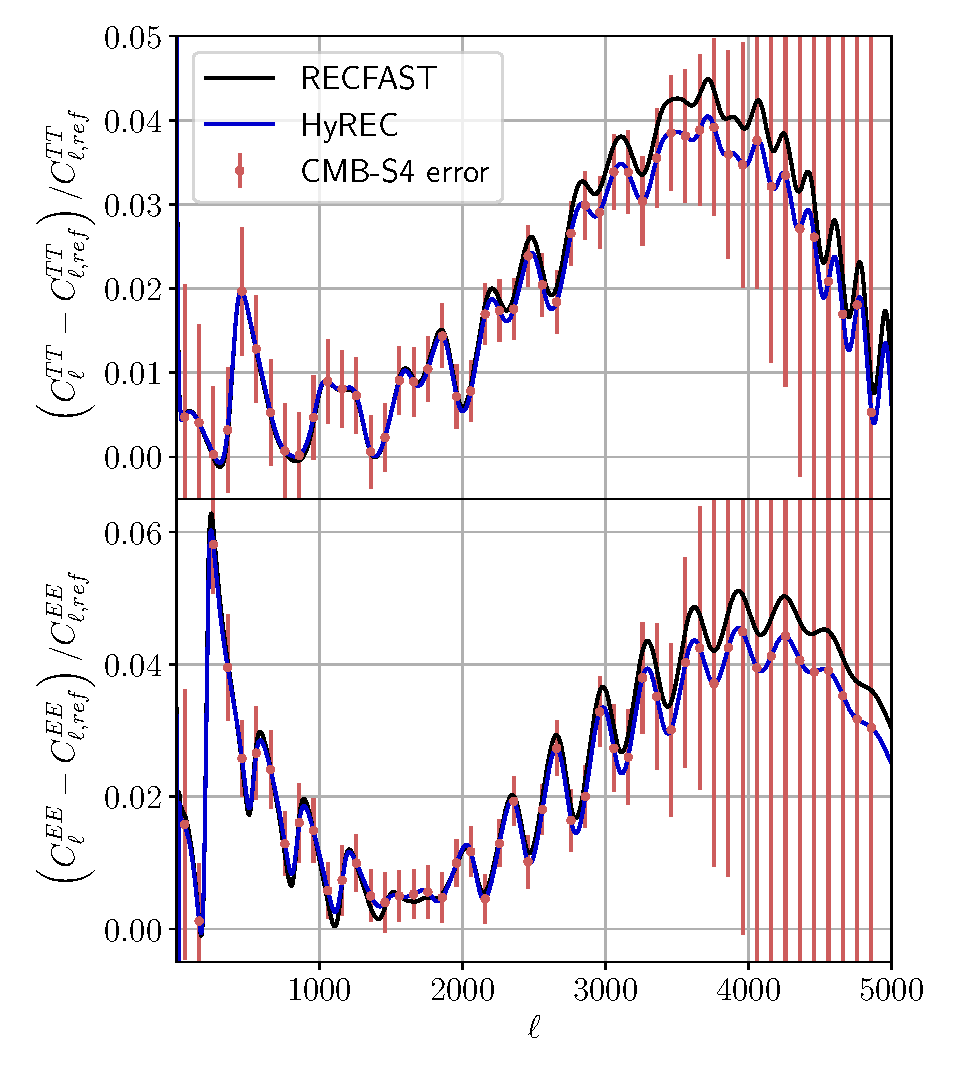
\includegraphics[width=\columnwidth]{img/M3demo-reccodes.pdf}
\caption[Difference in CMB power spectrum multipoles computed with different recombination codes]{Relative shifts between $\Lambda$CDM with standard recombination (taken as reference $C_{\ell,\rm ref}$) and a particular M3 configuration ($\delta_-=-0.9$, $\delta_+=5/3$, $f_0=1/3$ giving $b=1$, like in \cref{fig:M3demo-damping}), using RECFAST (in black) and HyREC (in blue).
The red bands correspond to CMB-S4 errors binned with $\Delta\ell=100$.
The cosmological parameters ($\theta_s$, $\omega_b$, $\omega_\mathrm{cdm}$, $A_s$, $n_s$, $\tau_\mathrm{reio}$) are fixed to the Planck best fit. }
\label{fig:M3demo-reccodes}
\end{figure}

In the main text we used the recombination code RECFAST, as it is faster than the more precise HyREC; here we justify that this choice does not bias our results.
RECFAST is sufficiently accurate for the analysis of {\it Planck} data, though this code will not be satisfactory for future CMB missions \citep{hyrec2}.
Moreover, highly nonstandard hydrogen densities, which can appear in the $\pm$ zones in M3, might limit the RECFAST applicability even further.

For our purposes, the change of zero-point is not the most important, as we focus on the shift introduced by clumping.
Therefore, we compare the relative changes in $C_\ell^{TT/EE}$ between $\Lambda$CDM with standard recombination and M3 with $b=1$ clumping obtained with RECFAST and HyREC (with full hydrogen model) in \cref{fig:M3demo-reccodes}.
We overlay the CMB-S4 error bars to assess the difference.
There is no notable difference for $\ell\leq 2000$-2500, so for current {\it Planck} data both codes can be considered equivalent.
In particular, the differences between each M3 model and $\Lambda$CDM are $\Delta\chi^2_{Planck,\rm RECFAST}=93$ and $\Delta\chi^2_{Planck,\rm HyREC}=90$, which are very close (as we note we have not shifted any parameters here).
For SO or CMB-S4, however, the difference between the recombination codes can be larger. 
For the lines shown, $\Delta\chi^2_{\rm CMB-S4,RECFAST}=1350$ and $\Delta\chi^2_{\rm CMB-S4,HyREC}=1150$, if one assumes the {\it Planck} best-fit cosmology (fixed), which shows a relative difference between the recombination codes of $\lesssim 20\%$.
Near the fiducial, where most of posterior is, the absolute difference will naturally be lower.
Also, for CMB-S4 precision the shifts in parameters are expected to be less than $1\sigma$ \citep{hyrec2}.
We conclude that an analysis of real SO and CMBS4 data  should use HyREC, though RECFAST is sufficient for our forecasting purposes.

\subsection{Neutrino masses}
\label{sec:justify-mnu}

\begin{figure}[ht!]
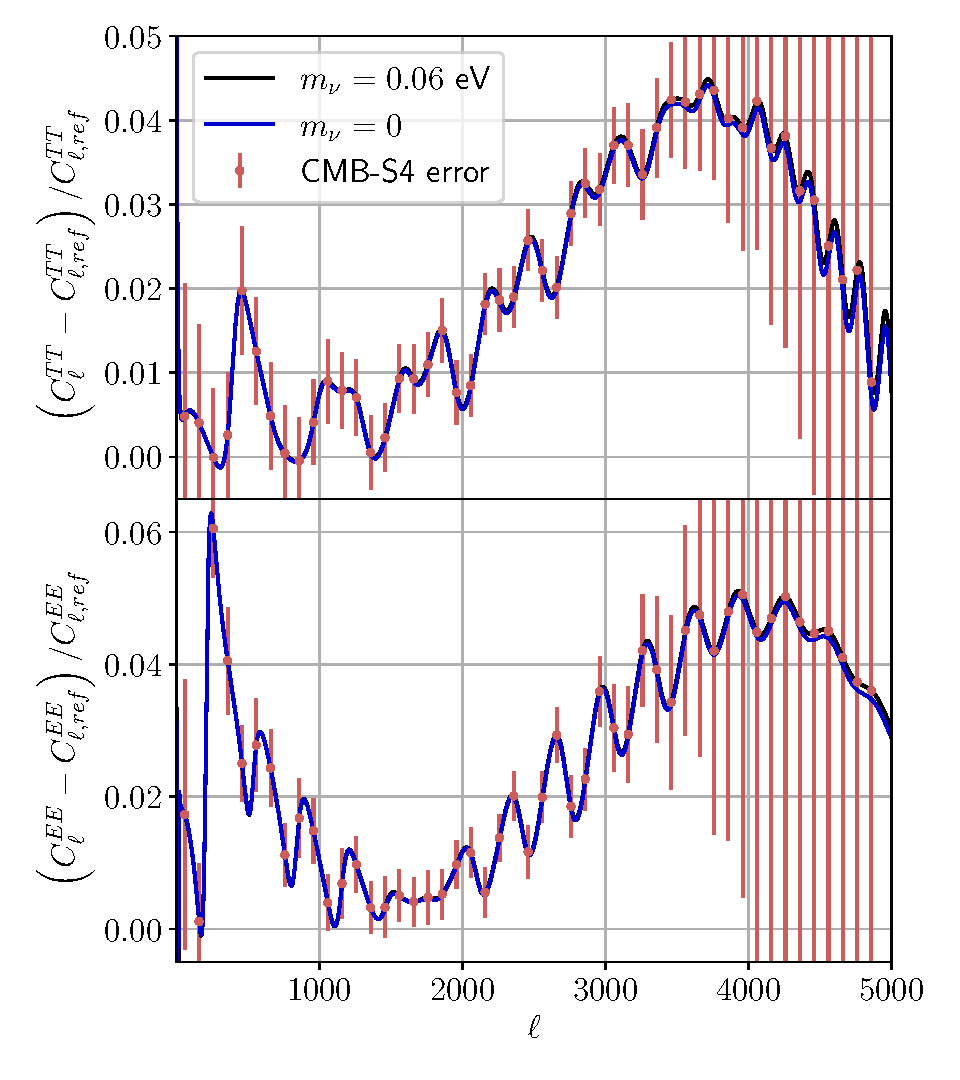
\includegraphics[width=\columnwidth]{img/M3demo-neutrinos.pdf}
\caption[Impact of massive neutrinos on CMB power spectrum multipoles]{Same as \cref{fig:M3demo-reccodes} but comparing the cases of massive (black) and massless (blue) neutrinos.}
\label{fig:M3demo-neutrinos}
\end{figure}

Throughout this paper we assumed massless neutrinos for efficiency, as it reduces the computational overhead by an order of magnitude. 
This increases our best fit $H_0$ compared to the {\it Planck} one.
However, again, we are most interested in changes introduced by clumping with respect to standard recombination, so we compare them for massive and massless neutrinos in \cref{fig:M3demo-neutrinos}.
The difference between both predictions in this plot is minuscule, and always smaller than even the CMB-S4 error bars.
More quantitetively, for the lines shown, $\Delta\chi^2_{Planck,m_\nu=0.06\,\rm eV}=92.6$ and $\Delta\chi^2_{Planck,m_\nu=0\,\rm eV}=93.3$; $\Delta\chi^2_{{\rm CMB-S4},m_\nu=0.06\,\rm eV}=1346$ and $\Delta\chi^2_{{\rm CMB-S4},m_\nu=0\,\rm eV}=1334$ (if one assumes {\it Planck} best fit cosmology for fiducial).
The relative difference in $\Delta\chi^2$ is $\lesssim 1\%$ in both cases.
Therefore computing with massless neutrinos suffices our purposes.

\section{Full contours from {\it Planck} runs}
\label{sec:fullcontours}

In \cref{fig:planckSH0ES-fullcontours} we show posteriors for all parameters in runs of M3 with {\it Planck} 2018 data (without and with SH0ES).
The posteriors on clumping parameters $\log_{10}\left(-\delta_-\right)$, $\log_{10}\left|\delta_+/\delta_-\right|$ and $f_0$ are largely flat, like the priors, except the decrease for higher $|\delta_-|$ for {\it Planck} and increase in the same place for {\it Planck}+SH0ES.
The clumping parameters also show almost no correlations with standard cosmological parameters, except a weak $H_0$ increase for the highest $|\delta_-|$.
Addition of SH0ES causes some increase in $n_s$, $\Omega_bh^2$, $H_0$; a weak increase in $A_s$ and $\tau_{\rm reio}$; some decrease in $\Omega_{\rm cdm}h^2$.

\begin{figure*}[ht!]
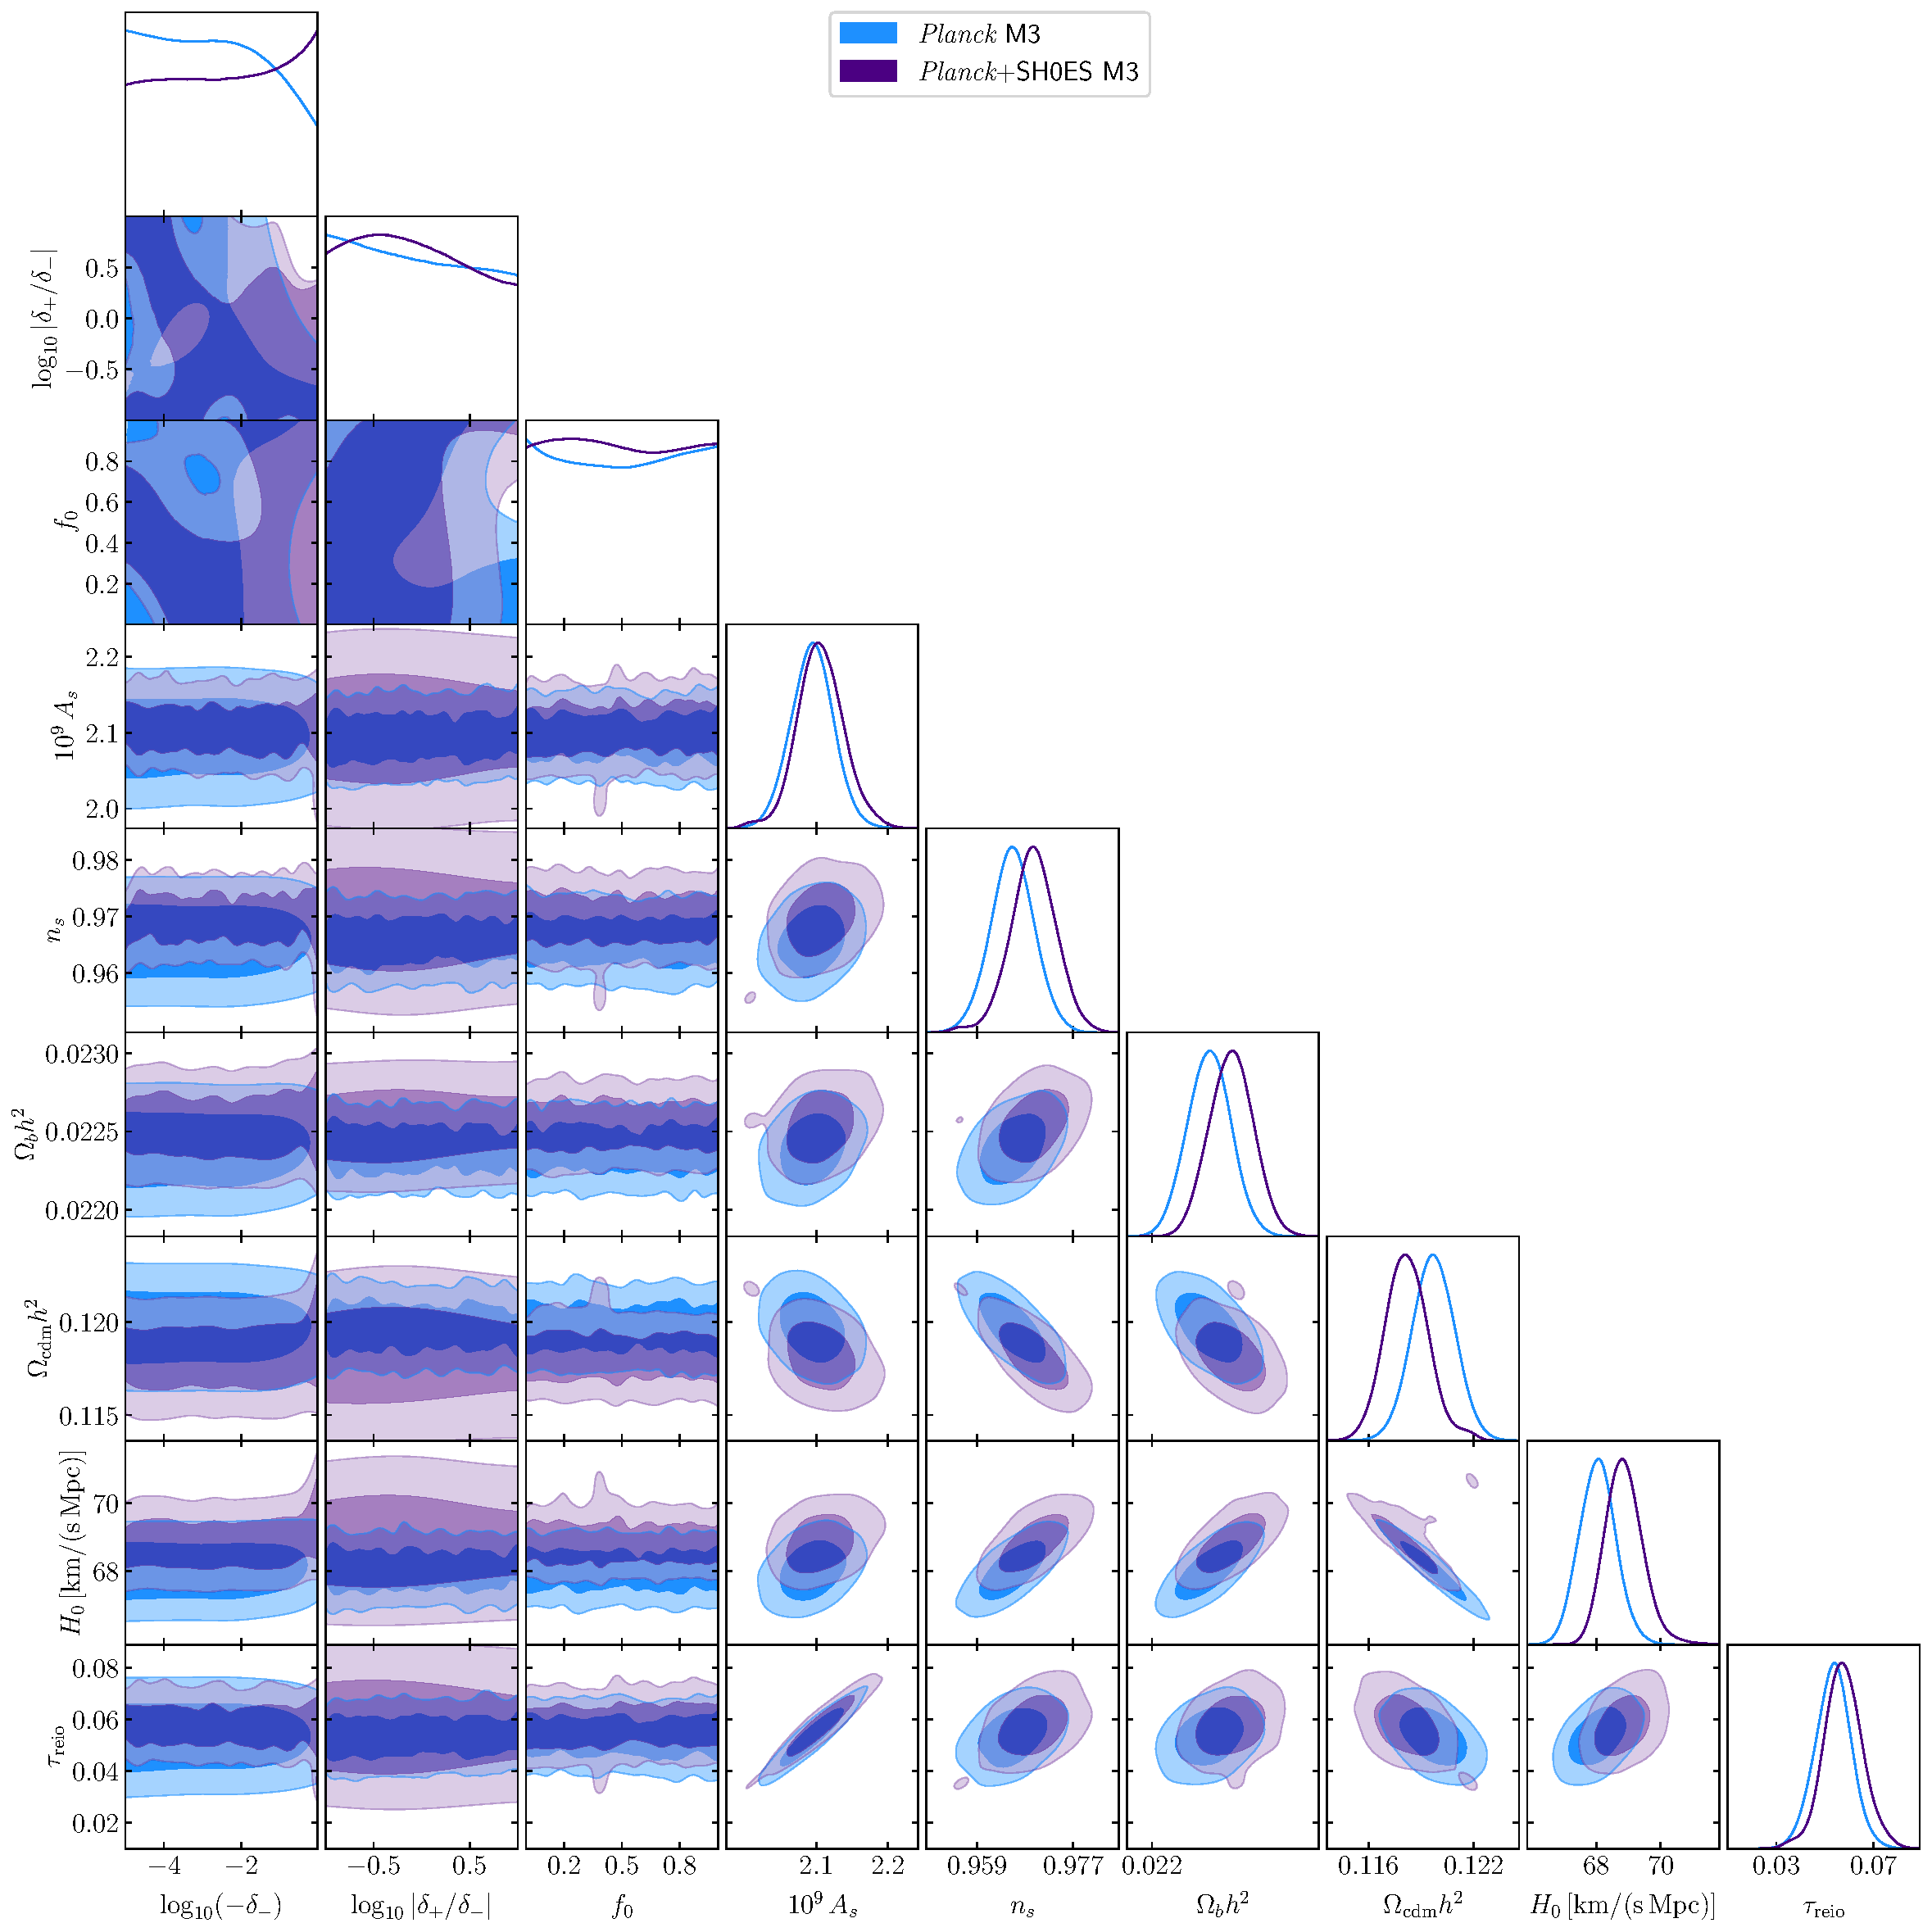
\includegraphics[width=\textwidth]{img/planckSH0ES-fullcontours.pdf}
\caption[Full contour plot for {\it Planck} runs of the clumping model.]{Full contour plot for {\it Planck} runs of M3. Purple is with SH0ES, blue is without.}
\label{fig:planckSH0ES-fullcontours}
\end{figure*}

\section{Best fit parameters}
\label{sec:bestfits}

\begin{table}[ht!]
\centering
\begin{tabular}{|c|c|c|c|}
\hline
Model & $\Lambda$CDM & $\Lambda$CDM & M3 \\
\hline
Fit to & {\it Planck} & \multicolumn{2}{c|}{{\it Planck}+SH0ES} \\
\hline
$\delta_-$ & n/a (0) & n/a (0) & $-$0.955 \\
$\delta_+$ & n/a (0) & n/a (0) & 1.320 \\
$f_0$ & n/a (1) & n/a (1) & 0.652 \\
\hline
$b$ & n/a (0) & n/a (0) & 0.439 \\
\hline
$10^9 A_s$ & 2.1094 & 2.1440 & 2.1132 \\
$n_s$ & 0.96604 & 0.97084 & 0.96552 \\
$100\theta_s$ & 1.04192 & 1.04207 & 1.04177 \\
$\Omega_b h^2$ & 0.022416 & 0.022569 & 0.022714 \\
$\Omega_\mathrm{cdm} h^2$ & 0.11945 & 0.11762 & 0.11999 \\
$\tau_\mathrm{reio}$ & 0.0514 & 0.0555 & 0.0542 \\
\hline
$H_0$ [km/(s Mpc)] & 68.146 & 68.993 & 70.916 \\
\hline
$\Omega_K$ & \multicolumn{3}{c|}{0} \\
$m_\nu$ [eV] & \multicolumn{3}{c|}{0} \\
\hline
$\chi^2_{{\rm low}\,\ell\,TT}$ & 23.2 & 22.4 & 23.6 \\
$\chi^2_{{\rm low}\,\ell\,EE}$ & 395.7 & 396.1 & 395.9 \\
$\chi^2_{{\rm high}\,\ell\,TTTEEE}$ & 582.2 & 584.0 & 585.4 \\
$\chi^2_{\rm lensing}$ & 9.0 & 8.7 & 8.8 \\
\hline
$\chi^2_{\it Planck}$ & 1010.0 & 1011.1 & 1013.7 \\
\hline
$\chi^2_{\rm SH0ES}$ & (15.1) & 10.5 & 3.1 \\
\hline
\end{tabular}
\caption{Our best fit parameters to (full) {\it Planck} and {\it Planck}+SH0ES.}
\label{tab:bestfits-planck}
\end{table}

In \cref{tab:bestfits-planck} we show the best fit parameters when fitting with full {\it Planck} data.
The M3 best fit to {\it Planck}-only is not shown, as we have not found a better one than $\Lambda$CDM, and the $\Lambda$CDM is included in M3 when one sets either one of the $\delta$'s to 0 or $f_0=1$.
Adding SH0ES in $\Lambda$CDM naturally increases $H_0$ as well as most input parameters: $A_s$, $n_s$, $\theta_s$, $\omega_b$, $\tau_\mathrm{reio}$; whereas $\omega_\mathrm{cdm}$ decreases slightly.
M3 allows for larger $H_0$, while the increase in $A_s$ and $\tau_\mathrm{reio}$ become smaller, $n_s$ and $\theta_s$ decrease very slightly, $\Omega_bh^2$ increases further than in $\Lambda$CDM and $\Omega_{\rm cdm}h^2$ increases, unlike in $\Lambda$CDM.
The CMB $\chi^2$ difference is dominated by high-$\ell$ $TT,TE,EE$ (where ``high'' means $\ell>30$).

\begin{table}[ht!]
\centering
\begin{tabular}{|c|c|c|c|}
\hline
Model & $\Lambda$CDM & $\Lambda$CDM & M3 \\
\hline
Fit to & {\it Planck} $\ell<1000$ & \multicolumn{2}{c|}{{\it Planck} $\ell<1000$ + SH0ES} \\
\hline
$\delta_-$ & n/a (0) & n/a (0) & $-$0.950 \\
$\delta_+$ & n/a (0) & n/a (0) & 1.196 \\
$f_0$ & n/a (1) & n/a (1) & 0.301 \\
\hline
$b$ & n/a (0) & n/a (0) & 0.794 \\
\hline
$10^9 A_s$ & 2.0918 & 2.1315 & 2.0705 \\
$n_s$ & 0.97026 & 0.97711 & 0.95944 \\
$100\theta_s$ & 1.04150 & 1.04179 & 1.04034 \\
$\Omega_b h^2$ & 0.022537 & 0.022773 & 0.022700 \\
$\Omega_\mathrm{cdm} h^2$ & 0.11831 & 0.11613 & 0.12198 \\
$\tau_\mathrm{reio}$ & 0.0518 & 0.0553 & 0.0505 \\
\hline
$H_0$ [km/(s Mpc)] & 68.528 & 69.640 & 72.616 \\
\hline
$\Omega_K$ & \multicolumn{3}{c|}{0} \\
$m_\nu$ [eV] & \multicolumn{3}{c|}{0} \\
\hline
$\chi^2_{{\rm low}\,\ell\,TT}$ & 22.4 & 21.4 & 24.8 \\
$\chi^2_{{\rm low}\,\ell\,EE}$ & 395.7 & 395.9 & 395.6 \\
$\chi^2_{{\rm high}\,\ell\,TTTEEE}$ & 286.3 & 288.2 & 281.5 \\
$\chi^2_{\rm lensing}$ & 8.9 & 9.0 & 8.8 \\
\hline
$\chi^2_{\it Planck}$ & 713.2 & 714.4 & 710.7 \\
\hline
$\chi^2_{\rm SH0ES}$ & (12.9) & 7.5 & 0.2 \\
\hline
\end{tabular}
\caption{Our best fit parameters to {\it Planck} $\ell<1000$, without and with SH0ES.}
\label{tab:bestfits-planck-lowl}
\end{table}

In \cref{tab:bestfits-planck-lowl} we show the best fit parameters when fitting with {\it Planck} $\ell<1000$ data.
The shifts in cosmological parameters are similar and small.
Interestingly, the addition of SH0ES helped to find a better fit to {\it Planck} than $\Lambda$CDM, unlike with {\it Planck}-only data.
This is likely because the optimal parameters region with high clumping is small.
However, the fit improvement is not significant.
The CMB $\chi^2$ difference is also dominated by high-$\ell$ $TT,TE,EE$ (where ``high'' now means $30<\ell<1000$).